\documentclass{sciposter}
\usepackage{poster-anppom}

% usar para termos estrangeiros
\newcommand{\eng}[1]{\textit{#1}}

\title{Taxonomia de Técnicas de Visualização em Música}
\author{\textbf{Jean Menezes da Rocha, Mara Pinheiro Menezes, Marcos
    da Silva Sampaio, Natanael Ourives, Dennis Queiroz de Carvalho e
    Pedro Ribeiro Kröger Júnior}} \institute{Genos---Grupo de pesquisa
  em computação musical} \email{jean.rudess@gmail.com}

% The following commands can be used to alter the default logo settings
\leftlogo[.7]{figs/ufba-logo}{% defines logo to left of title (with scale factor)
\rightlogo[1.1]{figs/capes-logo}  % same but on right

\begin{document}

\bibliographystyle{plain}

\conference{\Large \textbf{XII Congresso da ANPPOM --- 2012
    \hfill \textsf{Grupo de Pesquisa: GENOS}}}

\maketitle

\begin{multicols}{3}

\section{Introdução}

A visualização de informações tem auxiliado para o aumento da compreensão de
dados complexos em diversas áreas como estatística, estudos sociais, e música.
A visualização de dados em música pode abranger uma gama ampla de tópicos como
fuga, forma, contraponto, série dodecafônica, escalas, harmonia, e conjuntos de
notas, beneficiando leigos e profissionais e trazendo consigo potenciais
contribuições tanto a processos educacionais quanto a atividades terminais de
análise musical. Ainda assim, estudos mais rigorosos sobre a eficiência da
visualização não tem sido feitos e menos variáveis e mais objetivos os poucos
estudos indicam que a visualização pode auxiliar estudantes a aprender melhor o
material estudado.  Nosso objetivo neste trabalho é levantar formas mais
concretas e práticas de Visualização em Música. Dessa forma decidimos propor
uma taxonomia do que já tem sido implementado com tal finalidade.

\section{A ``Tabela Periódica de Métodos de Visualização''}

\section{Levantamento de técnicas de Visualização em Música}

O levantamento de técnicas consistiu em uma coleta bibliográfica, observação
das descrições de cada técnica trabalhada e catalogação da terminologia
relevante para o tema da pesquisa. As técnicas levantadas foram Visualização em
tempo real, Análise Harmônica, Análise Melódica, Visualização Preditiva,
Visualização de Coleções Musicais, e finalmente Ambientes integrados de edição
e visualização.

\subsection{Visualização em tempo real}

\subsection{Análises harmônica e melódica}

\subsection{Visualização preditiva}

\subsection{Visualização de coleções musicais}

\subsection{Ambientes integrados de edição e visualização}

\end{multicols}

\begin{multicols}{2}

\begin{figure}
  \centering
  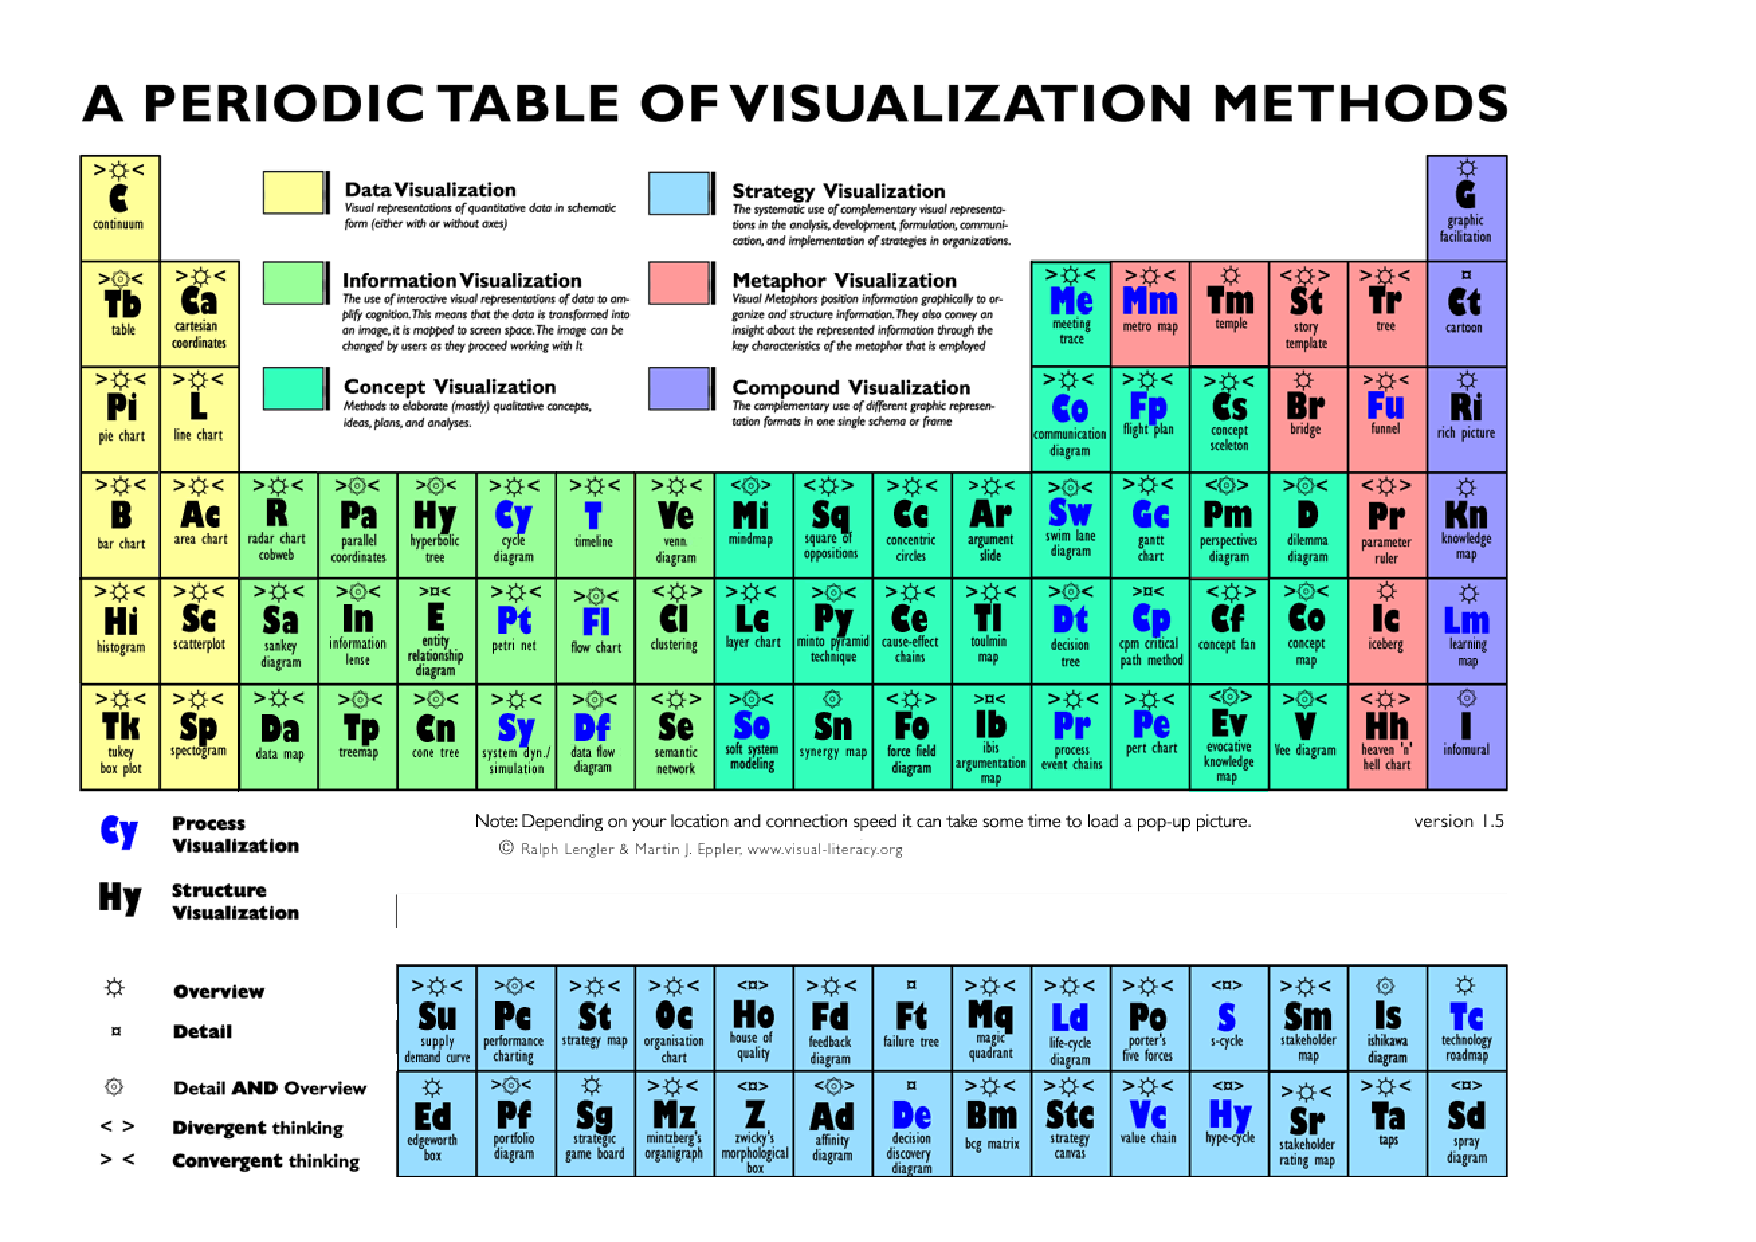
\includegraphics{./figs/tabela-periodica.pdf}
  \caption{Tabela Periódica de Métodos de Visualização \cite{Lengler2007}}
  \label{fig:label-figura}
\end{figure}

\begin{figure}
  \centering
  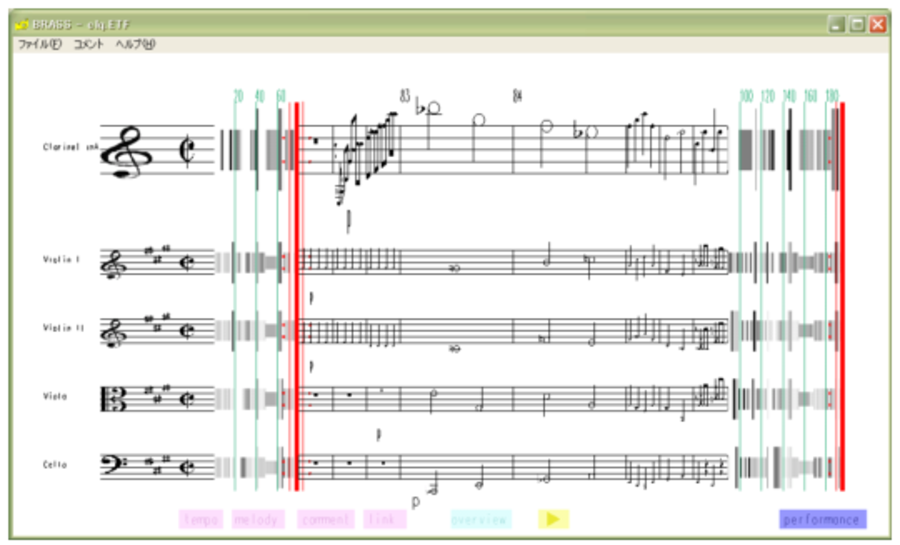
\includegraphics{./figs/watanabe-brass.pdf}
  \caption{Programa \textit{BRASS}, visualização em partitura condensada \cite{Watanabe2003}}
  \label{fig:label-figura}
\end{figure}

\begin{figure}
  \centering
  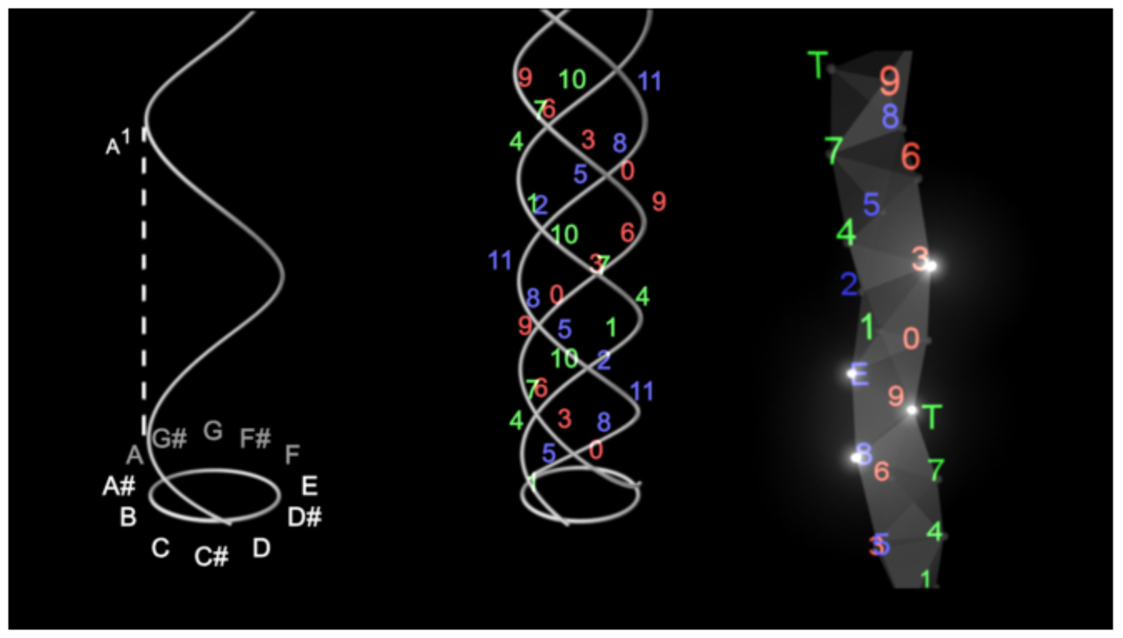
\includegraphics{./figs/bain-realtime.pdf}
  \caption{Visualização de análise harmônica automatizada \cite{Bain2008}}
  \label{fig:label-figura}
\end{figure}

\begin{figure}
  \centering
  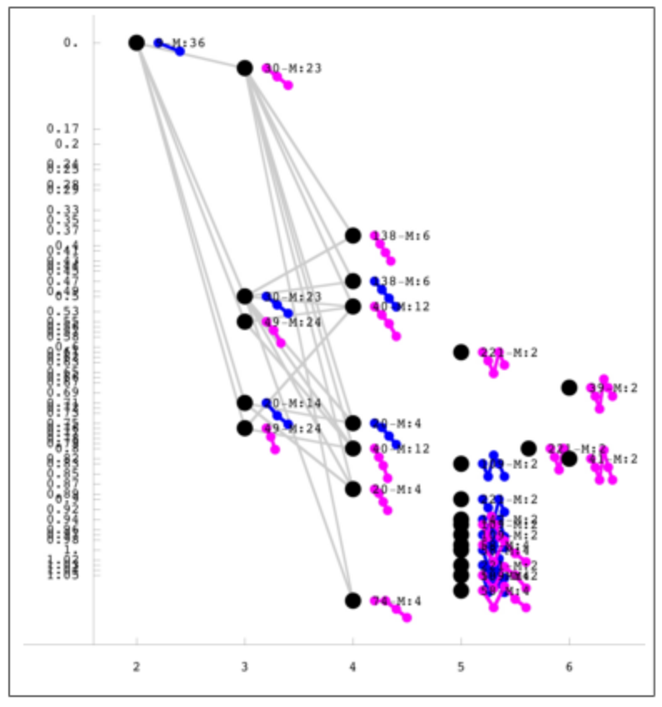
\includegraphics{./figs/buteau-motivic.pdf}
  \caption{Visualização de análise motívica automatizada \cite{Buteau2005}}
  \label{fig:label-figura}
\end{figure}

\begin{figure}
  \centering
  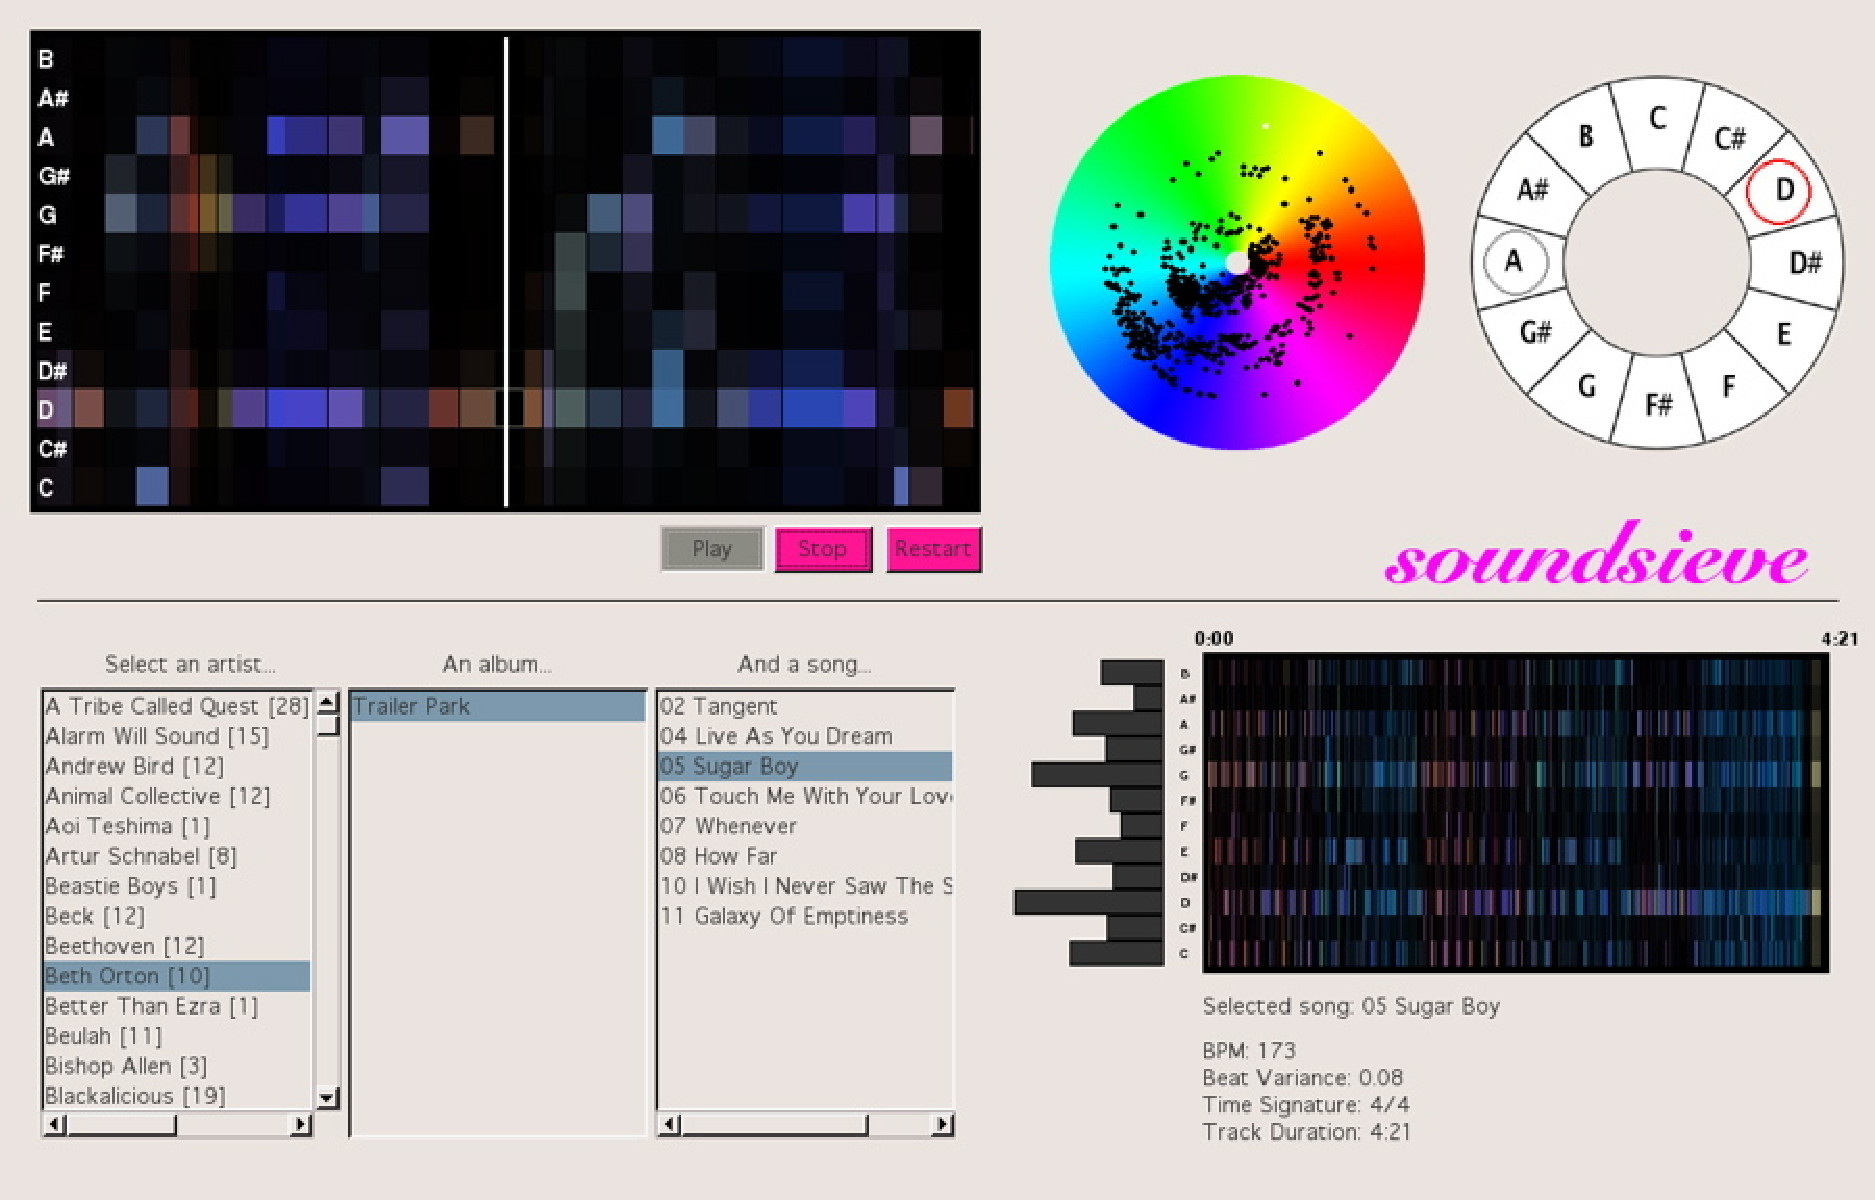
\includegraphics{./figs/soundsieve.pdf}
  \caption{\textit{Soundsieve}, disponível em \url{http://bit.ly/HvL7PK}}
  \label{fig:label-figura}
\end{figure}

\begin{figure}
  \centering
  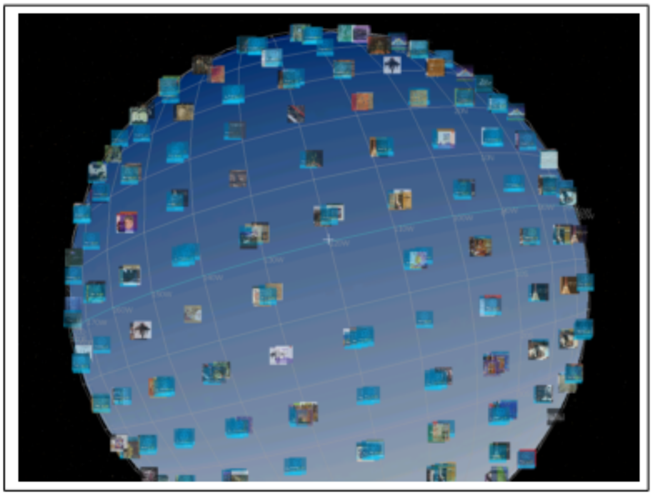
\includegraphics{./figs/topf-globe.pdf}
  \caption{Globe of Music \cite{Leitich2007}}
  \label{fig:label-figura}
\end{figure}

\begin{figure}
  \centering
  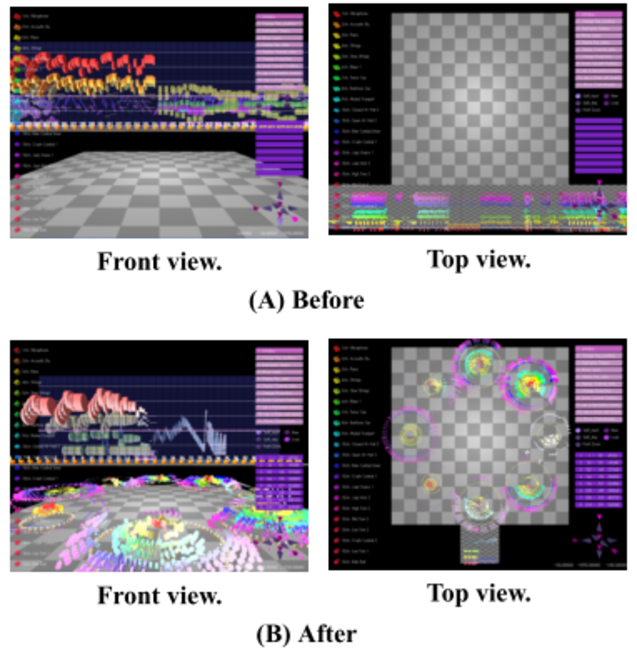
\includegraphics{./figs/comp-i.pdf}
  \caption{Programa \textit{comp-i} \cite{Miyazaki2004}}
  \label{fig:label-figura}
\end{figure}

\begin{figure}
  \centering
  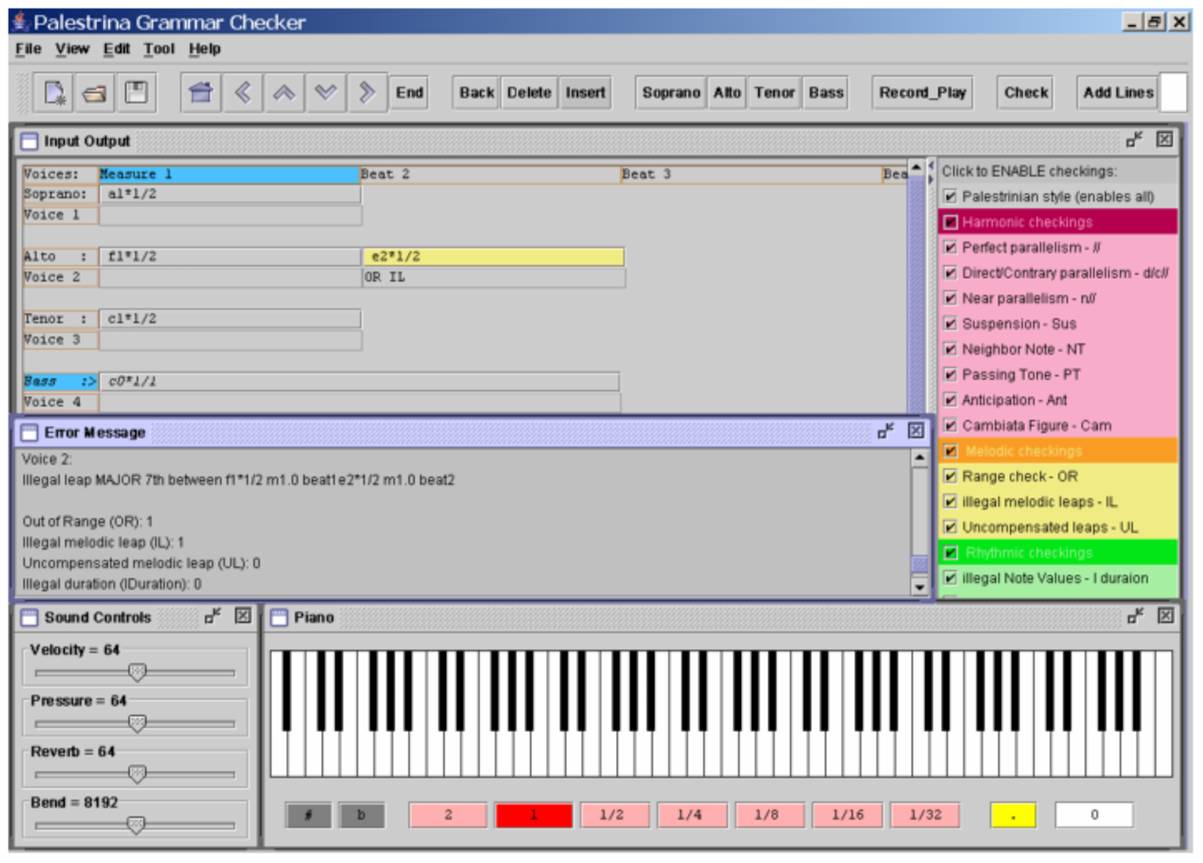
\includegraphics{./figs/palestrina-pal.pdf}
  \caption{Palestrina Pal \cite{Gramit2005}}
  \label{fig:label-figura}
\end{figure}

\end{multicols}

\begin{multicols}{3}

\section{Conclusão e trabalhos futuros}

A partir da coleta de informações, e de sua subsequente associação à taxonomia
de Lengler e Eppler constatamos que:

\begin{enumerate}
\item Todas as técnicas de Visualização pesquisadas possuíam ao menos uma das
propriedades associada à citada Tabela Periódica.
\item As técnicas investigadas concentram-se majoritariamente no campo de
Visualização de Informação, com um número significativo de técnicas também
situadas no campo de Visualização de Dados.
\item Os estudos de Visualização em Música estão mais focados com materiais e
instruções concretas e objetivas do que com procedimentos com maior nível de
abstração. Um possível indicativo é a presença de técnicas nos campos de
Visualização Composta e de Conceitos, e a ausência de técnicas em Visualização
de Metáforas e de Estratégias.
\item A avaliação objetiva de cada ferramenta apresentada ficou prejudicada pelo
fato de que nenhuma destas estava disponível para uso e/ou testes pelo público
em geral. A única fonte de pesquisa disponível consiste de artigos descritivos
das funções de cada ferramenta, mas não há versões acessíveis ou código-fonte
divulgado em quaisquer repositórios.
\end{enumerate}

Com esse trabalho observamos que a Taxonomia, a princípio comparativa, é um
ponto de partida determinante para a consolidação da Visualização em Música
como campo de estudo. No entanto é necessário verificar se a Visualização em
Música deve aderir aos princípios técnicos gerais da Visualização em caráter
permanente. A Visualização em Música ainda carece de técnicas para analisar
procedimentos em vez de materiais. Logo, deve-se considerar a hipótese de
surgimento de novas demandas técnicas ainda não cobertas pelos princípios mais
genéricos contemplados por esta taxonomia.

Além disso, não menos importante é a constatação de que as técnicas catalogadas
até agora parecem encerrar suas atividades apenas no âmbito de objetivos
parciais e práticas imediatas, sem necessariamente gerar uma contribuição
efetivamente compartilhada com a comunidade interessada. Para além de
relatórios sobre procedimentos arquivados de modo inacessível, entende-se como
fundamental a criação de ferramentas que possam ser disponibilizadas
publicamente, em condições de serem utilizadas por um grupo mais amplo de
pessoas -- mesmo aquelas que estejam fora de grupos e instituições acadêmicas.

\renewcommand{\refname}{Bibliografia}

\nocite{Lengler2007}

\bibliography{bibliography.bib}

\end{multicols}

\end{document}
